\documentclass[11pt]{article}

\usepackage[utf8]{inputenc}
\usepackage[T1]{fontenc}
\usepackage[margin=1in]{geometry}
\usepackage{array}
\usepackage{float}
\usepackage{tikz}
\usetikzlibrary{positioning,fit,calc}

\begin{document}

\section*{Visuals}
\begin{figure}[H]
\centering
\resizebox{\textwidth}{!}{%
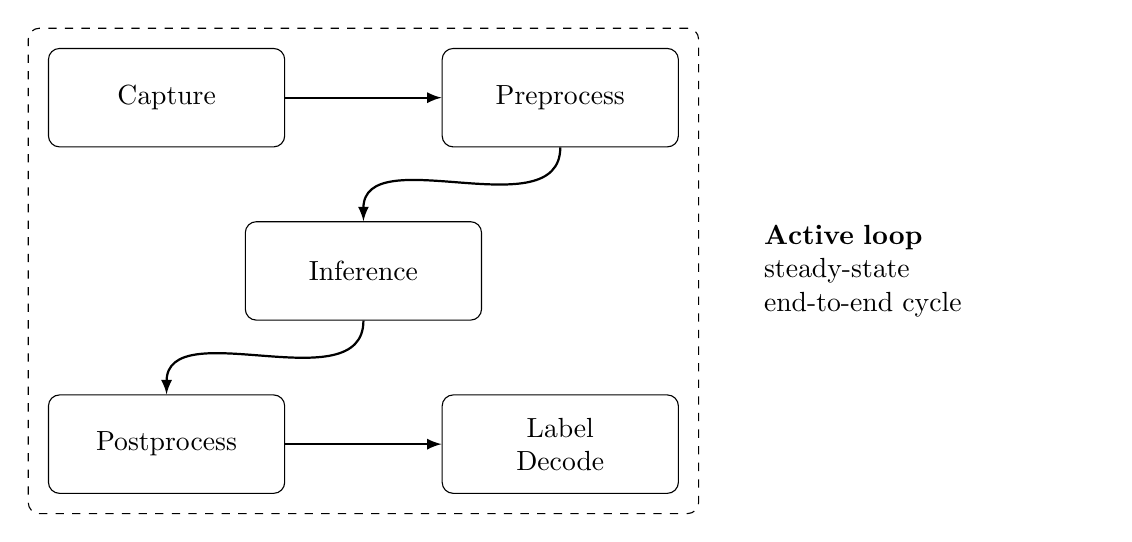
\begin{tikzpicture}[
  stage/.style={
    draw,
    rounded corners,
    align=center,
    minimum height=1.25cm,
    minimum width=3.0cm
  },
  loopbox/.style={
    draw,
    dashed,
    rounded corners,
    inner sep=0.25cm
  },
  looplabel/.style={
    align=left,
    text width=4.2cm
  },
  >=latex
]
\node[stage] (capture) at (0,0) {Capture};
\node[stage] (preprocess) at (5.0,0) {Preprocess};
\node[stage] (inference) at (2.5,-2.2) {Inference};
\node[stage] (postprocess) at (0,-4.4) {Postprocess};
\node[stage] (decode) at (5.0,-4.4) {Label\\Decode};
\node[loopbox, fit=(capture)(preprocess)(inference)(postprocess)(decode)] (loopfit) {};

\draw[->, thick] (capture) -- (preprocess);
\draw[->, thick] (preprocess.south) to[out=-90,in=90] (inference.north);
\draw[->, thick] (inference.south) to[out=-90,in=90] (postprocess.north);
\draw[->, thick] (postprocess) -- (decode);
\node[looplabel, right=0.7cm of loopfit.east] {\textbf{Active loop}\\steady-state\\end-to-end cycle};
\end{tikzpicture}
}
\caption{Sequential stages used for stage-by-stage latency profiling.}
\label{fig:runtime-stages}
\end{figure}
\begin{table}[H]
\centering
\large
\renewcommand{\arraystretch}{1.3}
\begin{tabular}{>{\raggedright\arraybackslash}p{5.6cm}rrr}
\hline
Metric & FP32 Baseline & FP16 & Delta \\
\hline
Capture mean (ms) & 4.950 & 2.512 & -49.25\% \\
Preprocess mean (ms) & 0.523 & 0.316 & -39.58\% \\
Inference mean (ms) & 268.395 & 60.493 & -77.46\% \\
Postprocess mean (ms) & 8.376 & 4.108 & -50.95\% \\
Label decode mean (ms) & 1.191 & 0.500 & -58.02\% \\
\textbf{Active loop mean (ms)} & \textbf{305.604} & \textbf{78.972} & \textbf{-74.16\%} \\
\textbf{Effective FPS} & \textbf{3.259} & \textbf{12.474} & \textbf{+282.75\%} \\
\hline
\end{tabular}
\caption{Sequential no-render FP32 vs.\ FP16 benchmark comparison.}
\label{tab:fp16-vs-locked-baseline}
\end{table}

\clearpage

\section*{Update Script}

For the systems and performance part of the project, our main progress so far has been building a reliable \textbf{stage by stage latency profiling} method, so we can justify speedup claims with trustworthy measurements. That means we split the pipeline into named sections, timed each section separately, and synchronized the GPU measurements so the numbers reflect the true cost of each stage.

That method helped us correct an earlier misleading bottleneck breakdown. Our first unsynchronized results made it look like postprocess was the main bottleneck, but after adding synchronized timing we found that inference was actually the dominant cost. Once we had that locked FP32 baseline, we added an FP16 inference path and reran the same benchmark scenario. On the current locked comparison, throughput improved from about 3.26 FPS to about 12.47 FPS, and steady-state active-loop latency dropped from about 306 milliseconds to about 79 milliseconds.

Over the next few weeks, the key performance improvements we plan to implement are:
\begin{itemize}
\item Create a backend-accelerated vision path, starting with TensorRT FP16 and moving to INT8 later.
\item Improve the Jetson camera-to-GPU path so live performance gains are not limited by the current demo-style OpenCV loop.
\end{itemize}

\section*{Reference Sections}
{\small \textit{Reference only: the sections below are for Q\&A and slide support. They are not intended to be read aloud unless someone asks how the profiling was done.}}

\subsection*{Performance Analysis Method}
This report uses \textbf{stage by stage latency profiling} with \textbf{synchronized timing}. The idea is simple: break the pipeline into named sections, measure each section separately, and compare the same workload before and after a change. In this project, CUDA synchronization is added around measured GPU stages so each timing reflects the real cost of that stage instead of delayed asynchronous work.

\subsection*{Measured Runtime Sections}


The benchmark runner separates the offline pipeline into the following measured sections so that bottlenecks can be attributed to a specific part of the runtime rather than to the loop as a whole.

\begin{itemize}
\item \textbf{Capture}: Time spent reading the next frame from the video source with OpenCV.
\item \textbf{Preprocess}: Time spent resizing frames, updating the temporal buffer, converting buffered frames into a tensor, and applying normalization before inference.
\item \textbf{Inference}: Time spent running the SiA vision path and computing similarity against the cached text embeddings.
\item \textbf{Postprocess}: Time spent converting raw model outputs into final detections after inference.
\item \textbf{Label decode}: Time spent mapping predicted label indices and scores into human-readable class names for display.
\item \textbf{Active loop}: Total time for one steady-state iteration where inference actually runs, excluding the early buffer-fill iterations.
\end{itemize}


\end{document}
